\documentclass[crop,tikz]{standalone}

\usepackage{amsmath}
\usetikzlibrary{decorations.markings}
\tikzset{>=latex}
\colorlet{green}{black!40!green}
\newcommand{\FZf}{\vec{F}_\text{Zf}}
\newcommand{\FZp}{\vec{F}_\text{Zp}}

\begin{document}
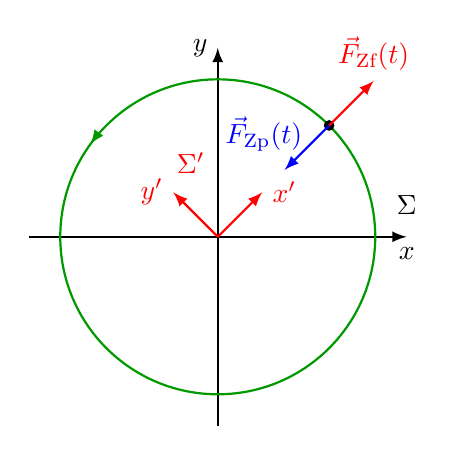
\begin{tikzpicture}[scale=2]
  \draw[->,thick] (-1.2,0) -- (1.2,0) node[below] {$x$};
  \draw[->,thick] (0,-1.2) -- (0,1.2) node[left] {$y$};
  \draw[->,red,thick] (0,0) -- (45:0.4) node[right] {$x'$};
  \draw[->,red,thick] (0,0) -- (90+45:0.4) node[left] {$y'$};
  \draw[
    decoration={markings, mark=at position 0.4 with {\arrow{>}}},
    postaction={decorate},
    green,
    thick
  ] (0,0) circle (1);
  \draw[fill] (45:1) circle (0.03);
  \draw[->,red,thick]  (45:1) -- +(45:0.4) node[above]{$\FZf(t)$};
  \draw[->,blue,thick] (45:1) -- node[left,xshift=0.2em,yshift=0.5em]{$\FZp(t)$} +(-135:0.4);
  \node at (1.2,0.2) {$\Sigma$};
  \node at (110:0.5) {\textcolor{red}{$\Sigma'$}};
\end{tikzpicture}
\end{document}
